\chapter{جمع‌بندی و انتقال تجارب کار گروهی}
در این فصل، تجریبات خودمان را از یک ترم کار تیمی برای شما می‌نویسیم تا شما اشتباهات ما را مرتکب نشوید و بتوانید بهتر کار تیمی انجام بدهید.
\section{تجربیات کار تیمی}
کار تیمی یکی از مهم‌ترین \lr{skill}‌هایی است که چه بخواهید چه نخواهید باید بلد بشوید. شما هم باید بتوانید یک تیم را رهبری کنید و هم بتوانید تحت رهبری کس دیگری کارتان را انجام بدهید.

اول از همه، کار تیمی هیچوقت بدون یک مدیر یا سرگروه خوب به پایان نمی‌رسد و اگر چنین کسی موجود نباشد، کار همیشه روی زمین می‌ماند و کل کار بسیار \lr{overwhelming} و خسته‌کننده می‌شود. اولین کاری که می‌کنید باید این باشد که یک مدیرگروه خوب برای تیمتان انتخاب کند. ویژگی‌های این مدیرگروه (حداقل برای این درس و پروژه): 
\begin{itemize}
	\item 
	خودش نسبت به درس آگاه و دانا باشد.
	
	این یعنی کسی از بین خودتان را برای کار تیمی انتخاب کنید که از همه درسخوان‌تر باشد و حوصله‌ی این درس را داشته باشد. وجود چنین کسی در سمت مدیرگروه باعث می‌شود که گروه بداند باید چه کاری را، چگونه انجام بدهد.
	در بزرگ‌ترین گروه‌ها یا مثال‌هایی از رهبری‌هایی که در طول تاریخ و البته \lr{scripted TV shows} و فیلم‌های سینمایی پیدا می‌شود، این مورد کاملا مشهود است که مدیرگروه یا مدیرتیم خودش از همه بیشتر به کار واقف است.
	
	\item 
	خودش بیشتر از همه برای پروژه تلاش کند.
	
	وظیفه‌ی یک مدیر تقسیم وظایف و دستور دادن نیست، اتفاقا مدیر \textit{در کنار همه‌‌ی این وظیفه‌‌های مدیریتی} باید خودش هم قسمتی از کار را انجام دهد. در این کار، او باید بتواند به دیگر اعضا در \lr{task}‌هاشان کمک کند.
	
	\item 
	مدیرگروه باید دارای مقبولیت و اقتدار باشد.
	
	مدیرگروه \textbf{باید} بتواند مسئولیت بدهد و نتیجه‌ را بخواهد. اگر چنین کسی نیستید بدانید یا کارتان پیش‌ نخواهد رفت یا همه‌ی مسئولیت‌ها به گردن شمای مدیرگروه خواهد افتاد. پس باید بتوانید مسئولیت بدهید و نتیجه را طلب کنید.
	
	\item 
	مدیرگروه باید مشاور خیلی خوبی باشد.
	
	از آنجایی که شما نمیتوانید و نباید همه‌ی کار‌ها را انجام بدهید و قبل‌تر هم اشاره شد که همه باید با هم کار کنید، اما شمای مدیرگروه باید بتوانید نظر خود و دیگران را در کار اصلی دخالت دهید؛ اینکار باعث بهتر و بهتر شدن نتیجه‌ی نهایی می‌شود ولی یادتان باشد که تصمیم آخر را خودتان باید بگیرید.
\end{itemize}

همین ۴ مورد را بتوانید انجام بدهید، گروه‌تان با مشکل مدیریتی مواجه نخواهد شد.

در طول رسیدگی به پروژه، هیچوقت هیچوقت کارتان را عقب نیندازید و هیچوقت نگذارید به هر دلیلی، وقفه‌‌ای در کارتان بیوفتد. (مثل تعطیلات عید :))
\section{ابزارات استفاده شده}
یکی از هیجان‌انگیزترین و جذاب‌ترین قسمت‌های این پروژه، ابزاراتی بود که استفاده کردیم، از ابزار‌های ارتباطی گرفته تا ابزار‌های مدیریت پروژه و برنامه‌ریزی و تقسیم وظایف.

اصولا برای کار حرفه‌ای باید بتوانید از ابزار‌های موجود و توسعه‌ داده شده توسط \lr{expert}ها و یا \lr{user}هایی که، مدت‌ها همان کار را کردند و برای راحتی خودشان ابزار‌هایی را توسعه دادند، استفاده کنید. چرا؟ خب این ابزارات دقیقا برای راحت‌تر کردن و بهتر کردن نتیجه‌ی کاری که می‌کنید توسعه و تست شدند و براحتی می‌توانند \lr{productivity} شما را چند برابر کنند و مهم‌تر از همه، باعث شوند تا روی پروژه و چیز‌های اصلی کارتان تمرکز کنید و باقی کار‌های ریز ولی مهم را به ابزارات بسپرید.

\subsection{نوشتن سند پروژه}
\subsubsection{نرم‌افزار حروف‌چین}
گروه ما، از ابزار حروف‌چینی 
\lr{\LaTeX }
و بسته‌ی 
\lr{\XePersian }
 برای حروف‌چینی و نوشتن پروژه استفاده کرد.
  
  این ابزار حروف‌چینی محبوبیت زیادی در بین دانشگاهیان دارد و دقیقا برای نوشتن و \textbf{نگهداری} چنین متونی استفاده می‌شود.
  
  از مزایای استفاده از \lr{\LaTeX } می‌توان به موارد زیر اشاره کرد
  \begin{itemize}
  	\item 
  	{\large استاندارد است.}
  	
  	در پروژه شما باید موارد نگارشی را به دقت رعایت کنید. به غیر از موارد نگارشی-نوشتاری مثل نیم‌فاصله:‌ می‌‌نویسم و نه می نویسم، دیگر نکات نگارشی مثل صفحه‌آرایی، تورفتگی‌ها و مواردی بسیار دیگری را، خود \lr{\LaTeX } برای شما رعایت می‌کند و شما فقط باید روی محتوایی که می‌نویسید دقت کنید.
  	\item 
    {\large روی همه‌ی سیستم‌عامل‌ها و حتی پلتفرم‌های آنلاین، به صورت رایگان در دسترس است.}
    
    \lr{\LaTeX }
     روی سیستم‌عامل‌های اصلی 
     \lr{Windows, Mac OS \& Linux} 
     براحتی و رایگان در دسترس است. این یعنی هر کسی در هر جایی و هر سیستم‌عاملی می‌تواند از این نرم‌افزار استفاده کند.
  	\item 
  	{\large انتقالش ساده‌ست}
  	
  	خروجی این نرم‌افزار از کامپایل یک فایل \lr{text} ساده بدست می‌آید. این به این معنی است اگر شما \lr{source code} و کامپایلر 
  	\lr{\LaTeX}
  	را داشته باشید می‌توانید، بنویسید، ویرایش کنید و خروجی بگیرید و این فایل ساده‌ی \lr{text} را براحتی هر جایی ذخیره و ویرایش کنید و نگران منتقل شدن آن از این سیستم به آن سیستم نباشید.
  	
  	\item 
  	{\large نگهداری با نرم‌افزار‌های ورژن}
  	
  	از آنجایی که \lr{source code} پروژه‌ی شما یک فایل \lr{text} است، میتوانید براحتی از نرم‌افزار‌های کنترل ورژن مانند \lr{git} برای مدیریت سندتان استفاده کنید.
  	
  	\item 
  	{\large خروجی خوب}
  	
  	خروجی گرفته شده از 
  	\lr{\LaTeX }،
  	 بسیار زیبا و استاندارد است. با تلاش کن شما بهترین و زیبا‌ترین خروجي را از 
  	 \lr{\LaTeX }
  	 دریافت می‌کنید. می‌توانید مثال‌های این بند را در خود همین داک مشاهده‌ کنید.
  	 
  	\item {\large امکانات جذاب}
  	
  	\lr{\LaTeX }
  	امکانات نوشتاری بسیار جذاب و قدرتمندی را در اختیار شما قرار می‌دهد که بسیاری از مشکلات نوشتاری شما را برطرف می‌کند.
  	
  	\begin{itemize}
  		\item فهرست مطالب
		
		تمام چیزی که به عنوان فهرست مطالب در اول این سند مشاهده می‌کنید فقط و فقط با یک دستور ایجاد شده و منِ نویسنده هیییییچ دخالتی برای تولید آن نداشتم. اگر دقت کنید که تمام شماره‌ صفحات درست هستند به هر خط دقیقا به همانجا لینک شده که با یک کلیک می‌توان به آنجا رفت.
		
		قسمتی از \lr{source code} سند که برای تولید فهرست مطالب استفاده شده است:
		
\begin{latin}
		\begin{lstlisting}
...
identifierstyle=\color{black}
}
% --------------------------------------------------

\begin{document}

\includepdf{title}
\frontmatter
\tableofcontents
\mainmatter

\chapter{سند نیازمندی‌ها}

\section{مقدمه}	
با توجه به افزایش روز افزون نرخ بیکاری در کشور ما کاریابی به صورت چشم‌گیر مورد توجه تمامی اقشار جامعه قرار گرفته است. بدین منظور ایجاد یک سامانه هدفمند برای کاهش این نرخ، سودمند است. سامانه نرم افزاری \textbf{کارتاپ}، با معرفی کارجویان به کارفرمایان و توانمندسازی افراد به منظور دریافت کار، این نیاز مهم را برآورده می سازد.

\subsection{هدف}
یکی از بزرگ‌ترین نیازهای جامعه امروز، یافتن شغل مناسب برای افراد است. در گذشته‌ای نه چندان دور، کارجویان برای پیدا کردن شغل، باید به دفاتر کاریابی مراجعه می‌کردند؛ اما مدتی‌ست که دیگر هر کاری از طریق اینترنت و به صورت آنلاین صورت می‌گیرد. با توجه به رقابت زیاد و اینترنتی شدن تمام امور، بهترین راه برای رفع این نیاز، طراحی پلتفرم کاریابی‌‌ای است که فضایی برای کارفرمایان و کارجویان فراهم می آورد تا بتوانند به راحتی به هدف خود برسند.
سامانه‌ی کاریابی به این صورت است که مشاغل را در دسته‌بندی‌های متفاوتی به کاربر نمایش می‌دهد و با استفاده از فیلترها، کارجویان میتوانند لیست مشاغل مد نظر خود را بیابند. همچنین برای سهولت کاربران امکان ساخت رزومه با قالب‌های حرفه‌ای و آماده را برای کارجویان فراهم می‌کند. کارفرما‌ها می‌توانند با پرداخت مبلغی، آگهی خود را روی سامانه قرار دهند تا به افراد جویای کار نمایش داده شود. همچنین کارفرماها می‌توانند مهارت‌های مورد نیاز برای موقعیت شغلی مورد نظر و همچنین، نوع کار از لحاظ پاره‌وقت، تمام‌وقت ، دورکاری و... را مشخص کنند.				علاوه بر موارد فوق این کار باعث شده تا نرخ بیکاری در کشور کاهش پیدا کند و افراد در کوتاه ترین زمان بتوانند شغل مورد نظر خود را پیدا کنند.

\subsection{قلمرو}			
این محصول که به نام کارتاپ شناخته می‌شود، بستری است که در آن متقاضیان کار می‌توانند شغل متناسب با مهارت‌های خود را جست‌وجو کنند و موقعیت‌های کاری مختلف را مقایسه کنند.
در کنار این موارد، بخش مهارت افزایی نیز وجود دارد که افراد می‌توانند با کسب آموزش‌های مورد نظر و کسب گواهی معتبر، خود را برای موقعیت‌های شغلی مختلف آماده کنند.

\subsection{تعاریف، سرنام‌ها و کوته نوشته‌ها}		
به جدول \ref{words} مراجعه شود.

\begin{sidewaystable}
	\begin{center}
		\caption{جدول واژگان، سرنام‌ها و کوته‌نوشته‌ها}
		\begin{tabular}{|c|c|p{9cm}|}
			
			\hline
			واژه &
			\centering واژه‌ی کامل &
			توضیح \\
			\hline
			\hline
			\lr{GPS} &
			
			\lr{Global Positioning System} &
			سامانه‌ای برای یافتن موقعیت جغرافیایی است. \\ 
			\hline
			
			\lr{HTTPS} & \lr{Hypertext Transfer Protocol Secure} &
			به معنای پروتکل انتقال ابر متنی است و وظیفه‌ی ‌ارسال و دریافت داده‌ها بین کلاینت و سرور را بر عهده دارد.\\ 
			\hline
			
			\lr{HTML} & \lr{Hypertext Markup Language} &
			زبان استایل دهی و ویرایش ویژگی‌های ظاهری محتوای صفحات وب می‌باشد. \\ 
			\hline
			
			\lr{CSS} & \lr{Cascading Style Sheets} & 
			زبان استایل دهی و ویرایش ویژگی‌های ظاهری محتوای صفحات وب می‌باشد. \\ 
			\hline
			
			\lr{SRS} & \lr{Software Requirement Specification} &
			به معنی مشخصات مورد نیاز نرم افزار می‌باشد.\\ 
			\hline
			
			\lr{CPU} & \lr{Central Processing Unit} &
			به معنی واحد پردازش مرکزی می‌باشد. \\ 
			\hline
			
			\lr{RAM} & \lr{Random Access Memory} &
			نوعی از حافظه‌ی کامپیوتری است که به هر ترتیبی قابل خواندن و تغییر است. \\ 
			\hline
			
			\lr{SSL} & \lr{Secure Sockets Layer} &
			فناوری امنیتی استاندارد برای برقراری یک پیوند رمزگذاری شده بین یک سرور و یک سرویس گیرنده می‌باشد. \\ 
			\hline
			
			\lr{PDF} & \lr{Portable Document Format} &
			فایل‌هایی هستند که برای باز کردن در وسائل مختلف به منظور مطالعه‌ی متن یا پرینت کردن آن به کار می‌روند. \\ 
			\hline
			
			\lr{SSD} & \lr{Solid State Drive} &
			به معنی درایو حالت جامد می‌باشد \\ 
			\hline
			
			\lr{UI} & \lr{User Interface} &
			نوعی فضایی است که تعامل میان انسان و ماشین در آن رخ می‌دهد \\ 
			\hline
			
			\lr{UX} & \lr{User Experience} &
			یک طراحی کاربر محور به این معناست که شما باید محصول یا خدماتی را ارائه بدهید که دقیقا همانکاری را انجام بدهد که کاربر می‌خواهد.  \\ 
			\hline
			
			\lr{JavaScript} & &
			یک زبان برنامه نویسی می‌باشد که به وسیله‌ی آن می توان بین کاربر و سایت ارتباط برقرار نمود. \\ 
			\hline
			
			کارجو & &
			شخصی است که به دنبال فرصت شغلی و کار می‌باشد. \\
			\hline
			
			کارفرما & &
			شخصی است که به علت نیاز نیروی انسانی در شرکتش، کارجویان را با توجه به مهارتشان و نیاز شرکتش، استخدام می‌کند \\
			\hline
		\end{tabular}\label{words}
	\end{center}
\end{sidewaystable}

\subsection{مراجع}\label{resources}		
\begin{latin}
	\lr{David Kung. $\ $ Object-oriented software engineering. $\,$  in \textit{An Agile Unified Methodology.} McGraw-Hill Higher Education, 2013.}
\end{latin}
\subsection{طرح کلی}		
روند کار در سند تدوین شده به این صورت است که در ابتدا اهداف و ویژگی‌های محصول شرح داده می‌شود و سپس به واسط‌های مختلف (من جمله واسط‌های سیستم، کاربر، سخت‌افزاری،نرم‌افزاری و...)، کارکردهای محصول ،مشخصات کاربران سیستم، قیود، مفروضات و وابستگی‌ها پرداخته و در نهایت به نیازمندی‌های آن خواهیم پرداخت.

\section{شرح کلی}
کارتاپ یک سیستم نرم‌افزاری برای کاریابی هدفمند در سازمان‌ها و شرکت‌هاست.
از طریق این سامانه، کارفرما نیاز‌های استخدامی خود را مطرح نموده و سپس بر اساس شغل و قابلیت‌های اعلام شده، بایستی بتواند به طور هوشمندانه کارجویان مناسب را به وی معرفی نماید. به نحوی می‌توان گفت این سیستم به منظور هوشمندسازی حداکثری روال‌های سنتی در این زمینه است.
از جمله امکانات این سیستم می‌توان به امکان ثبت نام کرفرما، ثبت اطلاعات شرکتی، اعلام نیاز استخدامی، ثبت آگهی و همچنین برای کارجویان، ایجاد پروفایل و رزومه شخصی اشاره نمود.

\subsection{چشم‌انداز محصول}
بر اساس سیستم مذکور درخواست‌های مورد نیاز برای کاربران با توجه به خواسته ارسال می‌شود و آن‌ها می‌توانند با بررسی درخواست‌ها و فایل‌های پیوست نظرات خود را اقدام کرده و در صورت نیاز با یک‌دیگر ارتباط بگیرند.
از جمله امکانات این سیستم دریافت رزومه، درخواست اخذ تست‌های بالینی برای کارفرمایان و همچنین شرکت در تست‌های شخصیت شناسی، ساخت رزومه شخصی، انتخاب علایق شغلی برای کارجویان اشاره کرد.

\subsubsection{واسط‌های سیستم}
واسط‌های سیستم این مسئله را بیان می‌کند که ارتباط سامانه‌ی ما با سیستم‌های خارجی، از طریق چه واسطه‌هایی صورت می گیرد و چگونه با هم در تبادل اطلاعات مختلف هستند. به عنوان مثال:
\begin{enumerate}
	\item
	دسترسی به پایگاه‌داده‌ی اداره‌ی ثبت احوال برای احراز هویت کارجو‌یان، مورد نیاز است.
	\item
	دسترسی به پایگاه‌داده‌ی اداره‌ی ثبت شرکت‌ها برای احراز هویت شرکت‌ها، مورد نیاز است.
	\item
	از آنجایی که این پلتفرم کاربران زیادی خواهد داشت، به سرور‌های قدرتمند و سریعی جهت پاسخ به درخواست‌ها و انجام عملیات‌های لازم، نیاز داریم.
	\item
	جهت ارتباط و اطلاع رسانی‌های مهم به کاربران از طریق پیامک، نیاز به ارتباط با سازمان‌های مخابراتی یا شرکت‌هایی‌ست که این نوع خدمات را ارائه می دهند.
\end{enumerate}

\subsubsection{واسط‌های کاربر}
جهت استفاده‌ی صحیح و کارآمد کاربران از سامانه، یک سری قابلیت‌های عمومی برای همگان و یک سری قابلیت‌های خاص در پنل کاربری کاربرانِ وارد شده در حساب کاربری، وجود دارد. در نتیجه نقش کاربران تعیین کننده‌ی سطح دسترسی آن‌ها می‌باشد. سطح‌ دسترسی یا نقش کاربران در این سامانه، به دو دسته تقسیم می شود:
\begin{enumerate}
	\item
	کارفرما
	\item
	کارجو
\end{enumerate}
\subsubsection{واسط‌های سخت‌افزاری}
واضح است سیستم نرم‌افزاری کاریابی، نیازهای سخت‌افزاری به‌خصوصی ندارد؛ با این وجود لیستی از واسط های سخت‌افزاری مورد نیاز اولیه در ادامه آمده است:
\begin{enumerate}
	\item
	ابزارهای اولیه جهت پردازش و مدیریت داده‌ها و عملیات:
	\begin{itemize}
		\item
		کارت شبکه
		\item
		مودم (اتصال اینترنت)
		\item
		سرور شبکه
		\item
		سرور پردازش داده
	\end{itemize}
	
	\item
	ابزار لازم برای پیدا کردن مکان دقیق شرکت‌ها:
	\begin{itemize}
		\item
		سرویس \lr{GPS}
	\end{itemize}
	
	\item
	دستگاه‌های موردنیاز جهت ارتباط افراد با بستر اینترنت (هر سخت‌افرازی که توانایی اجرای نرم‌افزارهایی نظیر مرورگرها را داشته باشد) مانند:
	\begin{itemize}
		\item
		تلفن همراه
		\item
		کامپیوتر شخصی
		\item
		تبلت
		\item
		لپ‌تاپ
	\end{itemize}
	
\end{enumerate}
\subsubsection{واسط‌های نرم‌افزاری}\label{software}
\begin{itemize}
	\item
	مرورگر‌های مرسوم همچون
	\lr{Google Chrome}،
	\lr{Mozilla Firefox} و
	\lr{Microsoft Edge}						که از آخرین نسخه‌های
	\lr{HTML}،
	\lr{CSS}						و
	\lr{JavaScript}						پشتیبانی می‌کنند.
	
	\item
	با توجه به حجم بالای داده‌ها، استفاده از سیستم‌های پایگاه‌ داده‌ی رابطه‌ای
	\LTRfootnote{Relational databases}
	و پایگاه‌داده‌های غیر رابطه‌ای
	\LTRfootnote{NOSQL databases}
	\item
	هر نرم‌افزاری که بتواند فایل با فرمت \lr{PDF} را نشان بدهد.
\end{itemize}
\subsubsection{واسط‌های ارتباطی}
این سیستم به صورت تحت‌ وب است که کاربران با توجه به نیاز‌ها با سرور و پایگاه داده ثبت احوال و اداره ثبت شرکت‌ها ارتباط گرفته تا احراز هویت شوند و کار مورد نظر خود را انجام دهند.

\subsubsection{واسط‌های حافظه}
از آنجا که در سیستم، لازم است اطلاعات ضروری کاربران که بخش اعظم جامعه را تشکیل می‌دهند، ذخیره و آمارگیری‌های مورد نیاز از طریق این داده‌ها استخراج شود، پس منطقی است که حافظه‌ی جانبی قابل توجهی به سیستم اختصاص یابد. همچنین در					پروسه‌ی تخصیص حافظه، نیاز سیستم به پردازش سریع داده‌ها در مراحل جستجو میان مشاغل در نظر گرفته شده ‌است.					پس به طور کلی:

\begin{enumerate}
	\item
	باتوجه به حجم پردازشی بالای این وب‌سایت جهت انجام امور مختلف، این سامانه نیازمند \lr{CPU}های قدرتمند و به‌روز و همچنین حافظه‌های عظیم و پرسرعت (همانند \lr{SSD}) است.
	
	\item
	همچنین از \lr{RAM}های قدرتمندی برای تسریع درخواست ها استفاده می‌شود.
\end{enumerate}
\subsubsection{واسط‌های عملیات}
\begin{enumerate}
	\item
	اطلاعات بین سامانه و پایگاه داده، به صورت خودکار تبادل می شود و به صورت دستی چیزی تغییر نمی‌یابد (مگر در صورت ایجاد مشکلی خاص.)
	\item
	برای این سامانه، نیاز به سرورهای قدرتمند و سریعی برای پردازش و ذخیره سازی داده‌ها نیاز است.
	\item
	مراحل اعتبارسنجیِ صحت اطلاعات ورودی و فیلترهای جست‌و‌جو به صورت خودکار، توسط سامانه انجام می‌شود.
	\item
	تمامی اطلاعات ویرایش شده یا بارگذاری شده، در همان لحظه
	صورت \lr{real time} \RTLfootnote{به سیستم‌‌‌هایی گفته می‌شود که به صورت بی‌درنگ و بدون نیاز به بارگذاری (\lr{reload}) مجدد صفحه‌، اطلاعات بروزشده نمایش داده می‌شوند؛ پیام‌رسان‌ تلگرام از بهترین مثال‌های این سیستم‌هاست.})	 در سرور‌های سامانه بروزرسانی یا بارگذاری می‌شوند.
	\item
	در صورت استفاده‌ی بیش از حد مجاز تعداد کاربران جهت متعادل سازی سامانه، باید از طریق هدایت ترافیک به چندین سرور، دسترسی به یک دامنه را آسان‌تر و سریع‌تر کرد.
	\item
	ارسال پیامک‌های انبوه به کاربران جهت اطلاع رسانی‌های مهم، به طور خودکار توسط سیستم‌های ارائه دهنده‌ی این نوع خدمات، انجام می‌شود.
	\item
	سامانه باید به صورت خودکار رزومه‌های کارجویان را با درخواست‌های شغلی کارفرمایان مقایسه کند و در صورت مطابقت به طرفین پیشنهاد دهد.
	\item
	سامانه باید مهارت‌های کارجویان را از رزومه‌های آن‌ها به طور خودکار استخراج کند.
	\item
	احراز هویت شرکت‌ها به صورت خودکار انجام شود.
\end{enumerate}

\subsubsection{نیازمندی‌های سازگاری با محیط نصب}
این سامانه روی تمامی دستگاه‌هایی که دارای مرورگر مورد نیاز در \ref{software} اشاره شده است، قابل اجرا می‌باشد و نیازی به نصب ندارد.

\subsection{کارکرد محصول}
این سیستم که به منظور سهولت در روند استخدام افراد در شرکت‌ها و یا پیدا کردن شغل توسط کارجویان طراحی شده‌ است، دارای قابلیت‌های متنوع برای هرکاربر می‌باشد:
\begin{enumerate}
	\item
	کارجویان
	\begin{itemize}
		\item
		کشف فرصت‌های شغلی
		\item
		معرفی شرکت‌ها و فرصت‌های شغلی موجود در هرکدام
		\item
		آگاهی از مشاغل جدید
		\item
		استفاده از فیلتر های پیشرفته برای یافتن مهارت، نوع ساعت کاری
		\item
		رزومه ساز آنلاین با قالب های پیشرفته و حرفه‌ای
		\item
		ارتباط آسان با کارفرمایان
		\item
		افزایش  مهارت‌های فردی کارجویان برای پیدا کردن شغل بهتر
		\item
		آموزش قوانین حقوقی به کارجویان برای جلوگیری هرچه بیشتر از کلاهبرداری‌های اینترنتی و شغلی
	\end{itemize}
	
	\item
	کارفرمایان
	\begin{itemize}
		\item
		جذب نیرو و درج آگهی استخدام
		\item
		امکان تحلیل و بهینه‌سازی آگهی با استفاده از آمار دقیق.
		\item
		مدیریت رزومه‌های دریافتی در پنل شرکت
		\item
		مدیریت وضعیت درخواست متقاضی از داخل سیستم و اطلاع‌دهی به کارجو.
		\item
		معرفی و تبلیغ برند
		\item
		جستجو در رزومه‌های دریافتی
		\item
		یادداشت گذاری بر روی رزومه‌ها
		\item
		انتشار رایگان آگهی‌ کارآموزی
	\end{itemize}
	
\end{enumerate}
از دیگر قابلیت‌های سیستم به موارد زیر میتوان اشاره کرد:
\begin{itemize}
	\item
	بخش مقالات و اخبار برای افزایش اطلاعات کاربران
	\item
	همگام با اصول بهینه سازی برای موتورهای جستجو
\end{itemize}

\subsection{مشخصات کاربر}
کاربران کارتاپ به دو دسته‌ی کارفرمایان و کارجویان تقسیم می شوند:

\begin{enumerate}
	\item
	کارجویان
	این دسته از کاربران شامل افرادی از جامعه هستند که در جست‌وجوی کاری مطابق با مهارت‌ها، استعدادها و یا مدرک تحصیلی خود با توجه به شرایطی همچون محل اقامت، میزان ساعات کاری و... می‌باشد. از این دسته افراد انتظار می‌رود که علاوه بر دسترسی به اینترنت، توانایی کار با مرورگر، ثبت نام، بارگذاری یا تشکیل رزومه، احراز هویت و همچنین آشنایی با زبان فارسی را داشته باشند.
	\item
	کافرمایان
	
	این دسته از کاربران شامل افراد یا شرکت‌هایی هستند که در صدد پذیرش یا استخدام کارجو می‌باشند. آنها پس از بررسی و پذیرش رزومه‌ی کارجویان، مهارت‌ها و شرایط موردنظر خود را با مشخصات کارجو سنجیده و در صورت تطابق، کارجو را استخدام می‌کنند. این دسته از کاربران علاوه بر انتظاراتی که از کارجویان می‌رود ،ملزم به دارا بودن کد ثبت شده‌ی شرکت و پروانه‌ی کسب نیز می‌باشند.
\end{enumerate}

\subsection{قیود}
\begin{enumerate}
	\item
	دسترسی به کارتاپ باید به صورت شبانه‌روزی برای کاربران فراهم باشد.
	\item
	واسط‌های کاربری کارتاپ باید شرایط آسان و قابل‌فهمی را برای کاربران فراهم سازد.
	\item
	کارتاپ باید در کمتر از ۱۸ ماه به مشتری تحویل داده شود.
	\item
	هزینه تحلیل، طراحی و توسعه‌ی کارتاپ مطابق بودجه پروژه باید حداکثر \lr{50,000,000,000} ریال باشد.
\end{enumerate}
\subsection{قوانین کسب‌و‌کار}
\begin{itemize}
	\item
	رمز شخصی به هنگام احراز هویت و رمز موقت برای هر بار ورود، به شماره تلفن همراهی که کاربر هنگام ثبت نام وارد میکند فرستاده می‌شود.
	\item
	با توجه به اجباری بودن بیمه، کارفرمایان موظف هستند که شرایط بیمه کردن کارجویان را فراهم سازند.
	\item
	استخدام کارجویان توسط کارفرمایان در چارچوب قوانین اداره کار صورت می‌پذیرد.
	\item
	هر کارفرما برای ثبت شرکت باید دارای کد تایید شده توسط سامانه ثبت شرکت‌ها باشد.
	
\end{itemize}
\subsection{مفروضات و وابستگی‌ها}
در این قسمت هر یک از عوامل موثر بر الزامات مندرج در \lr{SRS} که می‌توانند بر آن تأثیر بگذارند، آورده شده است:

\begin{enumerate}
	\item
	وابستگی‌ها
	\begin{itemize}
		\item
		به دلیل حجم بالای اطلاعات، سیستم به پایگاه داده‌های کلان داده وابسته است.
		\item
		اطلاعات پایگاه داده‌های اداره ثبت شرکت‌ها در جریان‌های کاری سیستم، مورد نیاز است.
		\item
		جهت ارتباط و اطلاع رسانی‌های مهم به کاربران از طریق پیامک نیاز به ارتباط با سازمان‌های مخابراتی یا شرکت‌هایی است که این نوع خدمات را ارائه می‌دهند.
	\end{itemize}
	
	\item
	مفروضات
	\begin{itemize}
		\item
		کاربر توانایی دسترسی به اینترنت و تسلط کار با آن را داشته باشد.
		\item
		کاربر از دستگاهی با قابلیت اتصال به اینترنت و اجرای مرورگر جهت استفاده از خدمات سامانه، برخوردار است.
		\item
		کاربر حداقل دانش مورد نیاز برای کار با دستگاه‌های هوشمند را دارد.
		\item
		مرورگر کاربر از جاوا اسکریپت پشتیبانی کند.
	\end{itemize}
\end{enumerate}

\section{نیازمندی‌های خاص}

\subsection{نیازمندی‌های واسط خارجی}
\begin{enumerate}
	\item
	سیستم داده‌هایی را از ثبت احوال می‌گیرد و پس از آن کارجویان را  احراز هویت می‌کند.
	\item
	سیستم کد مربوط به هر شرکت را، به اداره ثبت شرکت‌ها می‌فرستد و جواب احراز هویت شرکت‌ها را دریافت می‌کند.
	\item
	سیستم با ارتباط با سازمان‌های مخابراتی و شرکت‌های اپراتور همراه‌اول، ایرانسل و یا رایتل به کاربران پیامک‌هایی با موضوعاتی از قبیل ارسال کدتایید، اطلاع‌رسانی، اخبار و ... می‌فرستد.
\end{enumerate}

\clearpage
\subsection{نیازمندی‌های کارکردی}
برای فهم راحت‌تر و چیدمان بهتر، نیازمندی‌ها به سه دسته‌ی پلتفرم، کارجو و کارفرما تقسیم شده‌اند.
\RTLfootnote{این تقسیم‌بندی قرار نیست خیلی دقیق باشد، چون مفهوم مطالب در بعضی موارد خیلی بهم نزدیک هستند؛ این کار صرفا برای جداسازی موارد مشابه بهم صورت گرفته است.}

\begin{enumerate}
	
	\addeditem
	کارتاپ باید امکان ثبت درخواست برای آگهی‌های شغلی متفاوت را برای کارجو فراهم سازد.
	
	\begin{enumerate}
		\subr 
		کارتاپ باید به هنگام ثبت درخواست کارجو، امکان وارد کردن حقوق پیشنهادی وی را فراهم کند
	\end{enumerate}
	
	\addeditem
	کارتاپ باید امکان نشاندار کردن و ذخیره کردن آگهی‌ها را برای کارجویان فراهم سازد.
	
	\addeditem
	کارتاپ باید آگهی‌های پیشنهادی مطابق با اطلاعات کارجو را نمایش دهد. 
	
	\addeditem
	کارتاپ باید قسمتی را به عنوان صفحه شخصی کارجو شامل پروفایل، اطلاعات شخصی، علایق و دسته‌بندی مشاغل داشته باشد.
	
	\addeditem
	کارتاپ باید امکان تغییر اطلاعات پروفایل کاربری و رمز عبور را داشته باشد.
	
	\addeditem
	کارتاپ باید قسمتی را به عنوان پنل کاربری اختصاص دهد.
	
	این بخش برای نمایش آخرین وضعیت و روند تمامی درخواست‌ها، شامل موارد زیر می‌باشد:
	
	\begin{itemize}
		\item
		ارسال شده
		\item
		در حال بررسی
		\item
		دیده شده توسط کارفرما
		\item
		تأیید یا رد درخواست
		\item
		علل تایید یا رد درخواست
	\end{itemize}
	
	\addeditem
	کارتاپ باید توانایی ایجاد و ویرایش رزومه‌ی الکترونیکی (رزومه ساز) برای کارجویان را فراهم نماید.
	
	\addeditem
	کارتاپ باید قابلیت بارگذاری فایل رزومه را برای کارجویان فراهم نماید. 
	
	\addeditem
	کارتاپ باید قسمتی را برای نمایش روند تمامی پیشنهادهای دیگر کارفرمایان برای استخدام کارجو اختصاص دهد. 
	
	\addeditem
	کارتاپ باید آگهی‌های فوری و آگهی‌های پیشنهادی را برای کارجو نمایش دهد.
	
	
	\addeditem
	کارتاپ باید امکان جستحو و یا فیلتر کردن آگهی‌ها بر حسب زمان نشر آنها و همچنین  مواردی از قبیل نام استان و شهر، نوع مهارت‌ها و انتخاب نوع موقعیت شغلی را برای کارجویان فراهم سازد.
	
	\addeditem
	کارتاپ باید امکان فرستادن رزومه به چندین آگهی به صورت همزمان را داشته باشد. 
	
	
	\addeditem
	کارفرما باید امکان ثبت آگهی شغلی را در این سیستم داشته باشد.
	
	\addeditem
	کارتاپ باید امکان ثبت‌نام شرکت‌ها را براحتی در اختیار کارفرما‌یان قرار دهد.
	
	\addeditem
	کارتاپ باید امکان بارگذاری تصاویری از محیط کاری،فضای شرکت و... را برای کارفرمایان فراهم کند. 
	
	\addeditem
	کارتاپ باید امکان بارگذاری موقعیت مکانی شرکت توسط کارفرما را فراهم سازد.
	
	\addeditem
	کارتاپ باید بتواند کارجویان مناسب و مطابق با شرایط آگهی‌های شرکت‌ها را یافته و آنان را به کارفرما‌ها پیشنهاد دهد.
	
	\addeditem
	کارتاپ باید امکان وارد کردن اطلاعاتی نظیر شرایط کاری، دستمزد، جنسیت و انتظارات عمومی و تخصصی از سوی کارفرما را فراهم کند.
	
	\addeditem
	کارتاپ باید یک صفحه مربوط به اطلاعات شرکت، پرسنل شرکت، آگهی‌های فعال، آگهی‌های منقضی شده، تصاویر، درخواست‌های کارجویان و پیشنهاد‌های ارائه شده به کارجویان برتر را به طور کامل نمایش دهد.
	
	\addeditem
	کارتاپ باید امکان ایجاد اکانت پرمیوم و خرید اشتراک برای کارفرمایان جهت ثبت بیش از 10 آگهی و همچنین ایجاد دیگر امکانات را فراهم کند.
	
	\addeditem
	کارتاپ باید برای ثبت نام کارجویان، اطلاعاتی را از قبیل نام و نام‌خانوادگی، تلفن همراه و ایمیل را از کاربر دریافت نماید.
	
	\addeditem
	کارتاپ باید هنگام ثبت درخواست کارجو، عملیات احراز هویت کارجو (دریافت کد ملی و بررسی صحت آن، فرستادن کد تایید موقت برای تایید شماره تلفن) را فراهم کند
	
	\addeditem
	کارتاپ باید امکان ورود به سامانه را برای کاربران فراهم سازد.
	
	\begin{enumerate}
		\subr
		کارتاپ باید امکان بازیابی رمز عبور کاربر را در صورت فراموشی، از طریق شماره همراه و یا ایمیل ثبت شده در سامانه فراهم کند.
		
		\subr
		کارتاپ باید برای هر رمز موقت، اعتبار ۱ دقیقه ای قائل شود و بعد از این زمان رمز منقضی شود.
	\end{enumerate}
	
	\addeditem
	کارتاپ باید برای ایجاد آگهی استخدامی توسط کارفرما، عملیات احراز هویت، شامل: 
	\begin{itemize}
		\item نام شرکت
		\item	 شماره‌ی ثبت شرکت یا شماره ملی شرکت
	\end{itemize}
	را داشته باشد.
	
	\addeditem
	سامانه باید قابلیت چت آنلاین را با کارشناس مربوطه برای کاربر فراهم نماید. 
	\addeditem
	کارتاپ باید امکان خارج شدن از سامانه را برای کاربر فراهم کند.
	
\end{enumerate}
\subsection{نیازمندی‌های کارایی}
\begin{enumerate}
	\item
	سامانه باید توانایی پاسخ گویی هم زمان ۱۰۰۰۰ کاربر را داشته باشد.
	\item
	سامانه باید برای ورود کاربران از کد \lr{CAPCHA}
	\RTLfootnote{\lr{CAPCHA} یا همان کپچا، نرم‌افزاری آنلاین برای تولید سوالات و آزمون‌هایی‌ست که انسان به‌راحتی قادر به پاسخ‌گویی به آنهاست ولی کامپیوتر‌ها در حال حاضر، قادر به تشخیص و پاسخ به آنها نیستند. عبارت \lr{CAPCHA} مخفف عبارت \lr{Completely Automated Public Turing Test To Tell Computers and Humans Apart} است.}
	استفاده کند تا از اینکه فرد وارد شده ربات نباشد، اطمینان حاصل کند.
	\item
	سامانه باید برای ثبت نام کاربران با استفاده از کد احراز هویت، هویت افراد را تایید نماید.
	\item
	سیستم پیامکی سامانه باید بتواند پیامک‌ها را حداکثر ظرف ۲۰ ثانیه برای کاربران ارسال کند.
	\item
	سامانه باید طراحی کاربرپسند داشته باشد.
	\item
	کارتاپ باید در هرگونه مواجه شدن با خطا، چه از سمت کاربر و چه از سمت سرور، اخطار را با جزئیات گزارش دهد، تا نیروهای فنی این مورد را در اولین زمان ممکن بازبینی و رفع کنند.
	
\end{enumerate}

\subsection{قیود طراحی}
\begin{enumerate}
	\item
	امکان بارگیری رزومه‌ها به فرمت \lr{PDF} برای کاربران فراهم باشد.
	\item
	سامانه باید بر روی تمامی مرورگر‌های مرسوم همچون
	\lr{Google Chrome}،
	\lr{Mozilla Firefox} و
	\lr{Microsoft Edge}  قابل اجرا باشد.
\end{enumerate}

\clearpage
\subsection{صفت‌های سیستم‌ نرم‌افزاری}
\begin{enumerate}
	\item امنیت
	\begin{itemize}
		\item استفاده از قابلیت‌های پنل کاربری، فقط باید توسط کاربران احراز هویت شده، قابل دسترسی باشد.
		\item سامانه باید حافظ اطلاعات شخصی کاربران باشد.
		\item سامانه باید قابلیت پشتیبان‌گیری از اطلاعات سایت، که شامل اطلاعات کابران هم می‌شود و همچنین توانایی بازیابی اطلاعات را داشته باشد.
		\item به جهت افزایش و پایداری امنیت ارتباط سرور با سیستم کاربر، از پروتکل‌های امنیتی مانند \lr{SSL} و \lr{HTTPS} استفاده می‌شود.
		\item سامانه باید در صورت دریافت درخواست‌های بیش از حد مجاز اقدام به مسدود سازی کاربر به طور موقت کند.
		\item سامانه باید به طور لحظه‌ای اقدام به ذخیره‌ی اطلاعات تغییر یافته کند.
		\item سامانه باید در شرایط خاص خطاها را متوقف کند.
	\end{itemize}
	
	\item در دسترس بودن
	\begin{itemize}
		\item سامانه باید به طور شبانه روز به جز بازه‌ی اصلاحات دوره‌ای، قابل دسترسی باشد.
		\item
		سامانه باید از طریق تمامی مرورگر‌های مرسوم مانند
		\lr{Google Chrome}،
		\lr{Mozilla Firefox}،
		و
		\lr{Microsoft Edge}
		که از آخرین نسخه‌های
		\lr{HTML}،
		\lr{CSS}
		و
		\lr{JavaScript}
		پشتیبانی می‌کنند، در دسترس باشند.
		\item
		قابلیت مشاهده‌ی آگهی‌های استخدامی، حتی در صورت عدم ورود به حساب کاربری وجود داشته باشد.
	\end{itemize}
	
	\item پشتیبانی
	
	سامانه باید تیمی متشکل از پشتیبانان در زمینه‌های مختلف داشته باشد (به عنوان مثال پشتیبان فنی و پشتیبان روابط عمومی).
	
	\item رابط کاربری مناسب
	
	سامانه باید دارای رابط کاربری مناسب باشد. به طوری که هم دارای زیبایی های بصری باشد (\lr{UI}) و هم استفاده ی کاربر از آن ساده و معلوم باشد (\lr{UX}).
	
\end{enumerate}

\subsection{برنامه تکرار و برنامه‌ی مرحله}
جدول \lr{2.1} برنامه‌ی مربوط به تکرا‌ر‌های اجرای پروژه را ارائه نموده است.

\begin{table}[h]
	\caption{جدول برنامه‌ی تکرار}
		\begin{adjustbox}{width=\textwidth}
			\begin{tabular}{|c|c|c|c|c|}
				\hline
				نیازمندی & 
				وابستگی‌ها & 
				تکرار اول (۳ هفته) & 
				تکرار دوم  (۳ هفته) & تکرار سوم  (۳ هفته) \\
				\hline
				\hline
				\req{01} & \req{22} & 
				\zstar & & \\ \hline
				\req{02} & \req{23} & 
				\zstar & & \\ \hline
				\req{03} & \req{06} & 
				& \zstar & \\ \hline
				\req{04} & \req{23} & 
				\zstar & & \\ \hline
				\req{05} & \req{04} & 
				& \zstar & \\ \hline
				\req{06} & \req{23} & 
				\zstar & & \\ \hline
				\req{07} & \req{06}\lr{, }\req{04} & 
				\zstar & & \\ \hline
				\req{08} & \req{04} & 
				\zstar & & \\ \hline
				\req{09} & \req{06} & 
				\zstar & & \\ \hline
				\req{10} & \req{23} & 
				& \zstar & \\ \hline
				\req{11} & \req{23} & 
				& \zstar & \\ \hline
				\req{12} & \req{13} & 
				& & \zstar \\ \hline
				\req{13} & \req{14}\lr{, }\req{24} & 
				& & \zstar \\ \hline
				\req{14} & - & 
				& \zstar & \\ \hline
				\req{15} & \req{14} & 
				& & \zstar \\ \hline
				\req{16} & \req{14} & 
				& & \zstar \\ \hline
				\req{17} & \req{13}\lr{, }\req{21} & 
				& & \zstar \\ \hline
				\req{18} & \req{13} & 
				& & \zstar \\ \hline
				\req{19} & \req{13}\lr{, }\req{23} & 
				& & \zstar \\ \hline
				\req{20} & \req{14} & 
				& & \zstar \\ \hline
				\req{21} & - & 
				\zstar & & \\ \hline
				\req{22} & \req{23} & 
				\zstar & & \\ \hline
				\req{23} & \req{21} & 
				\zstar & & \\ \hline
				\req{24} & \req{23} & 
				& \zstar & \\ \hline
				\req{25} & \req{23} & 
				& \zstar & \\ \hline
				\req{26} & \req{23} & 
				& \zstar & \\ \hline
			\end{tabular}
		\end{adjustbox}
	\end{table}

...
		\end{lstlisting}
	\end{latin}
می‌بینید که فقط یک دستور \texttt{tableofcontents} هست که تمام فهرست مطالب این سند را تولید کرده است.

  		\item مراجع
  		
  		اشاره به منابع در اسناد علمی دارای استاندارد‌های خاصی است که همه‌‌ی ریزکاری‌های رفرنس‌دهی شما به مراجعتان را \lr{\LaTeX } به سادگی انجام می‌دهد. نمونه‌ی رفرنس‌دهی در این سند را در \ref{resources} مشاهده می‌کنید.
  		
		\item جداول
		
		تولید جداول و استفاده از جداول در این پروژه بسیار مهم است، و \lr{\LaTeX } از بهترین و منعطف‌ترین نرم‌افزار‌ها برای تولید جداولی پیچیده‌ست. می‌توانید جداول زیادی را در این سند پیدا کنید.
		
		\item رفرنس دهی
		
		رفرنس‌دهی به قسمت‌های مختلف سند و لینک کردن رفرنس کار بسیاری راحتی‌ست، برای مثل بخش \nameref{expandeds} دارای چندین رفرنس به چند جدول مختلف در صفحات مختلف است.
		
		\item صحفه‌‌آرایی

\lr{\LaTeX }
دارای \lr{template}‌های مختلف و تنظیمات پیش‌فرض صفحه‌‌آرایی‌ست که خروجی استانداری برای شما تولید می‌کند.
		\item شماره‌ی صفحات
	
		همانند تولید فهرست مطالب، \lr{\LaTeX } تمامی شماره صفحه‌ها به سبک‌های مختلف را به درستی برای شما تولید می‌کند و شما هیچ نگرانی برای این قسمت هم ندارید :)
		(به شماره‌ صفحه‌ی تولید شده در فهرست مطالب و فصل اول دقت کنید.)
		
  		\item شمارنده‌ها
  		
  		 اعداد شمارشی که در این داک تولید شده‌اند، تماماً توسط خود نرم‌افزار محاسبه شدند و هیچ‌کدام دستی نیستند. برای مثال اعدادی که در
  		 \ref{senario-counter} می‌بینید، همه‌ این اعداد \lr{dynamic} تولید شده‌اند و با حذف و یا افزون گام‌ها خودشان آپدیت می‌شوند. یا اعدادی که در جداول فصل \nameref{senario-table} مشاهده می‌کنید.
  		   		
  	\end{itemize}
  \end{itemize}
  
  \textbf{نکته‌ی مهم}:
  
  برای پروژه، شما وقتی برای \underline{یادگیری} \lr{\LaTeX } ندارید و اگر از قبل بلد نیستید بهتر است سراغش نیایید، چون بالاخره یک سری کلک‌ها، قلق‌ها و روش‌ها هست که به مرور زمان یاد می‌گیرید و وسط نوشتن پروژه اصلا جای این کار نیست. اگر به این نکته توجه نکنید، نه تنها \lr{\LaTeX } کمکی به شما نمی‌کند بلکه بدجور شما را اذیت خواهد کرد.

\subsection{نگهداری و مدیریت سند پروژه}
اشاره شد که مزایای استفاده از \lr{\LaTeX } چیست، اما در این قسمت این موضوع را بررسی می‌کنیم که چگونه این سند را نگهداری و مدیریت کردیم.

اگه شما تجربه‌ی برنامه‌نویسی در اندازه‌ی یک پروژه‌‌ی متوسط داشته باشید متوجه این شده‌‌اید که اصلا نمی‌توان با \lr{Ctrl-z} و امثالهم پروژه را مدیریت کرد. علاوه بر این بسیاری از کار‌هایی که نرم‌افزار‌‌های ورژن کنترل مثل \lr{Commiting, Branching, Log, ...} را بدون این نرم‌افزار‌ها نمی‌توانید که داشته باشید.

به همین منظور برای مدیریت 
\lr{source code}
 این پروژه‌، از نرم‌افزار \lr{git} استفاده گردید.
 بخشی از \lr{log} پروژه را می‌توانید اینجا مشاهده کنید:
 \begin{figure}[H]
 	\caption{خروجی \lr{\texttt{\$ git log --oneline}}}
 	\begin{center}
 		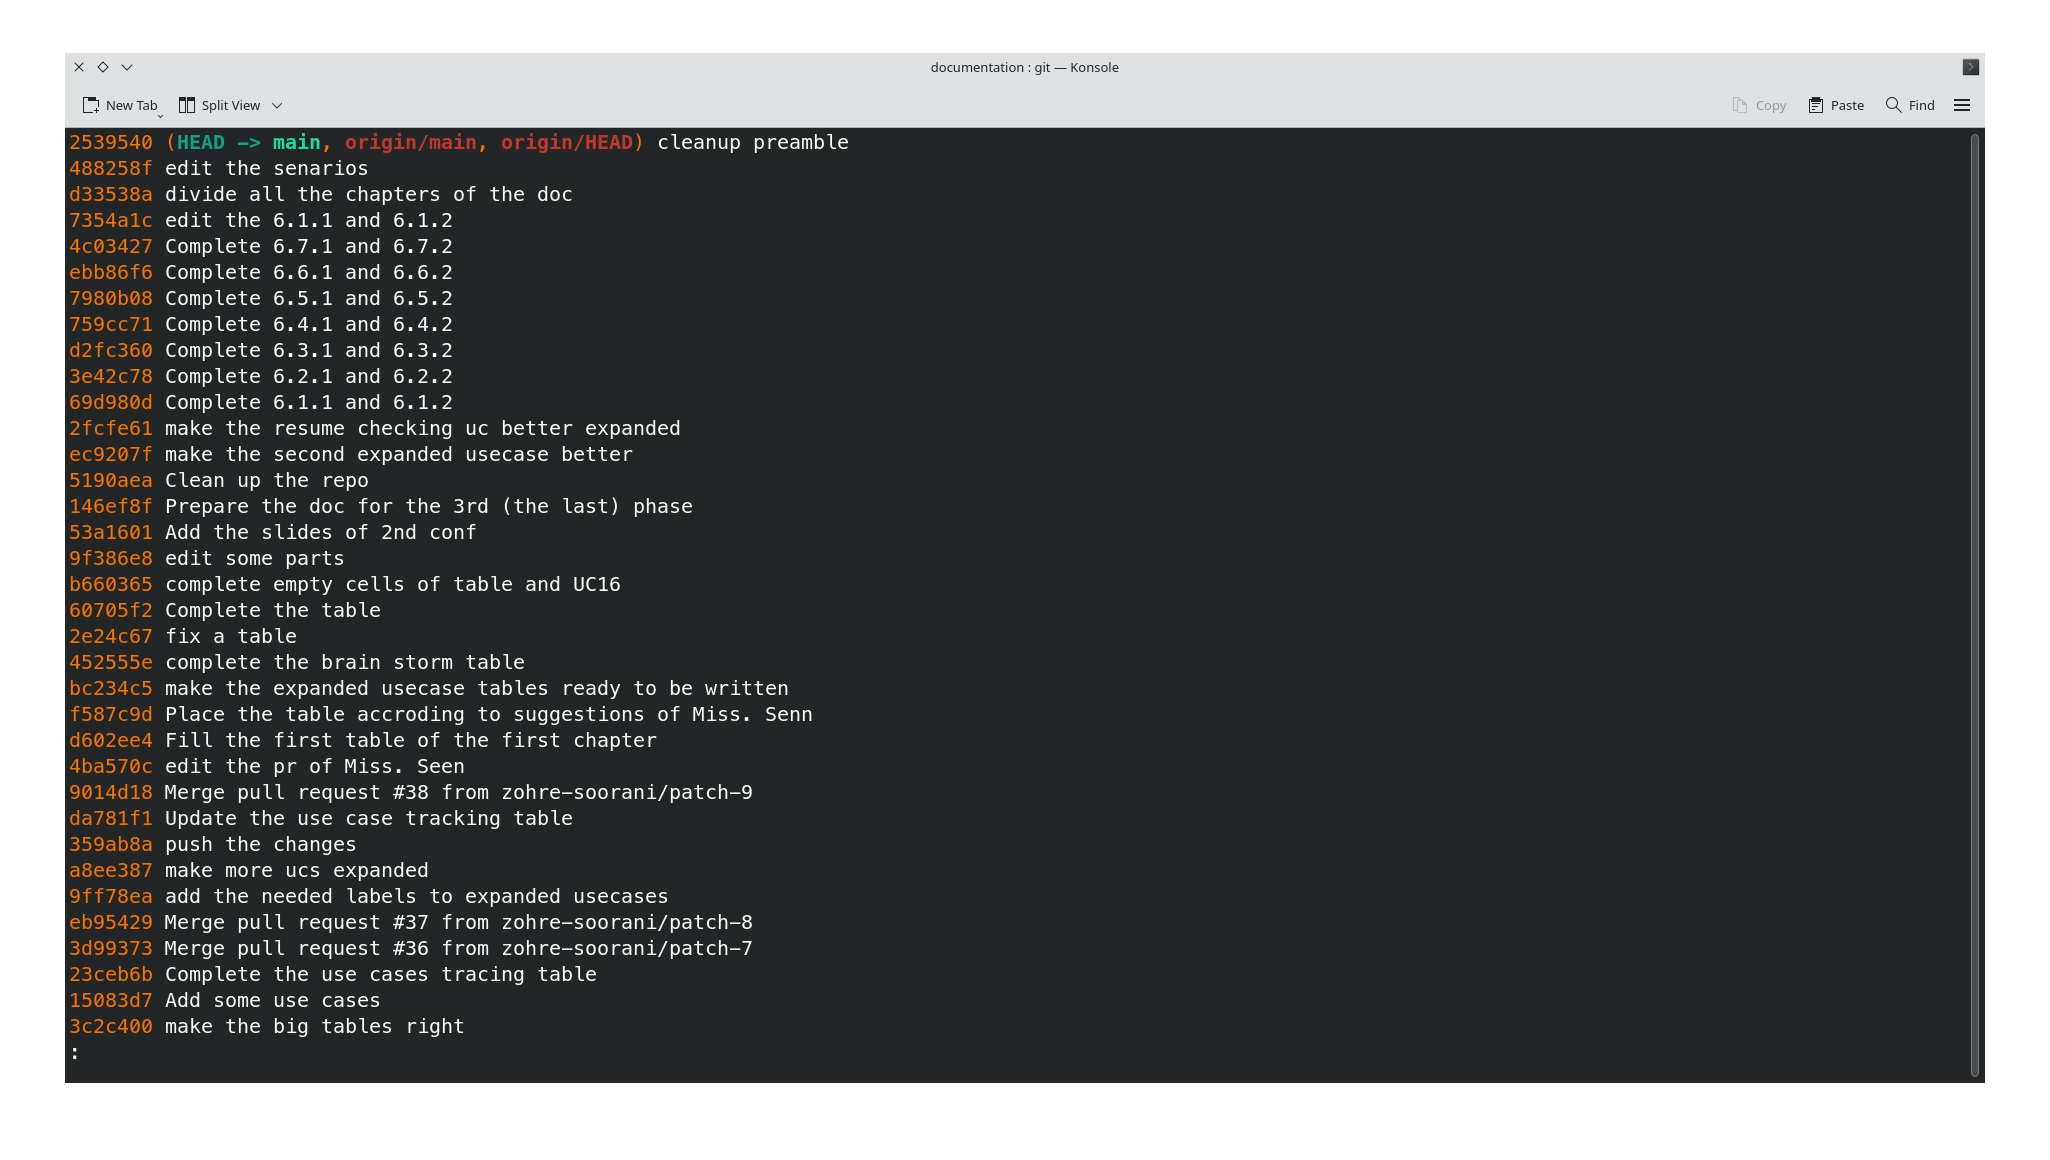
\includegraphics[angle=90, width=\textwidth, height=\textheight]{./images/log}
 	\end{center}
 \end{figure}

\subsubsection{کشیدن اشکال لازم پروژه}
تقریبا یک نرم‌افزار جهانی برای کشیدن تمام اشکال مورد نیاز شما در دنبا پیدا می‌شود که اسمش \lr{Visual Paradigm} است.
نصب ساده‌ای دارد و براحتی کرک می‌شود؛ می‌توانید برای نصب از این لینک \lr{\url{https://downloadly.ir/software/programming/visual-paradigm/}} استفاده کنید.
 
 اما برای کار‌های سبک‌تر می‌توانید از نسخه‌ی رایگان این نرم‌افزار در \textbf{محیط وب} استفاده کنید:
 \begin{latin}
 	\url{https://online.visual-paradigm.com}
 \end{latin}

\subsection{نگهداری ابری پروژه و \lr{collaboration}}
هیچوقت به \lr{Hard Drive}تان اعتماد نکنید. هر چیزی از پروژه و اطلاعات مهمی را که دارید، همیشه در پلتفرم‌های ابری ذخیره کنید.

وقتی شما روی \lr{source code} کار می‌کنید و از \lr{git} استفاده می‌کنید کاملا طبیعی‌ست که از پلتفرم‌های ابری مدیریت پروژه مثل \lr{GitHub, GitLab \& BitBucket} استفاده کنید، ما هم برای پروژه تصمیم گرفتیم که از \lr{GitHub} استفاده کنیم.

استفاده از گیت‌هاب مزایای زیادی دارد:
\begin{itemize}
	\item 
	همیشه یک بک‌آپ قابل اطمینان از تمام چیزی که دارید، آنجا هست.
	
	\item 
	\lr{collaboration}
	و همکاری اعضای گروه برای نوشتن سند، بسیار راحت می‌شود و گیت‌هاب امکانات زیادی مثل 
	\begin{itemize}
		\item \lr{Pull Requests}
		\item \lr{Issues}
		\item \lr{Releases}
	\end{itemize}
را در اختیار شما قرار می‌دهد.
\end{itemize}

\subsection{نحوه و روند مدیریت و نگهداری و \lr{collaboration}}
برای مدیریت سریع و راحت این پروژه تصمیم بر این شد که ریپازیتوری پروژه فقط یک ادمین داشته باشد، ادمین ریپازیتوری کسی‌ست که کنترل کامل روی محتوای داخل ریپازیتوری دارد، این شخص بهتر است همان شخصی باشد که \lr{\LaTeX } بلد است و مسئول نوشتن سند است.

دیگر اعضای گروه، این ریپازیتوری را \lr{fork} می‌کنند و تغییراتی که می‌خواهند روی \lr{source code} انجام می‌دهند و به ریپو‌ی اصلی \lr{Pull  Request} می‌دهند.

\begin{figure}[H]
	\caption{صفحه‌ی \lr{Pull Requests}}
\begin{center}
	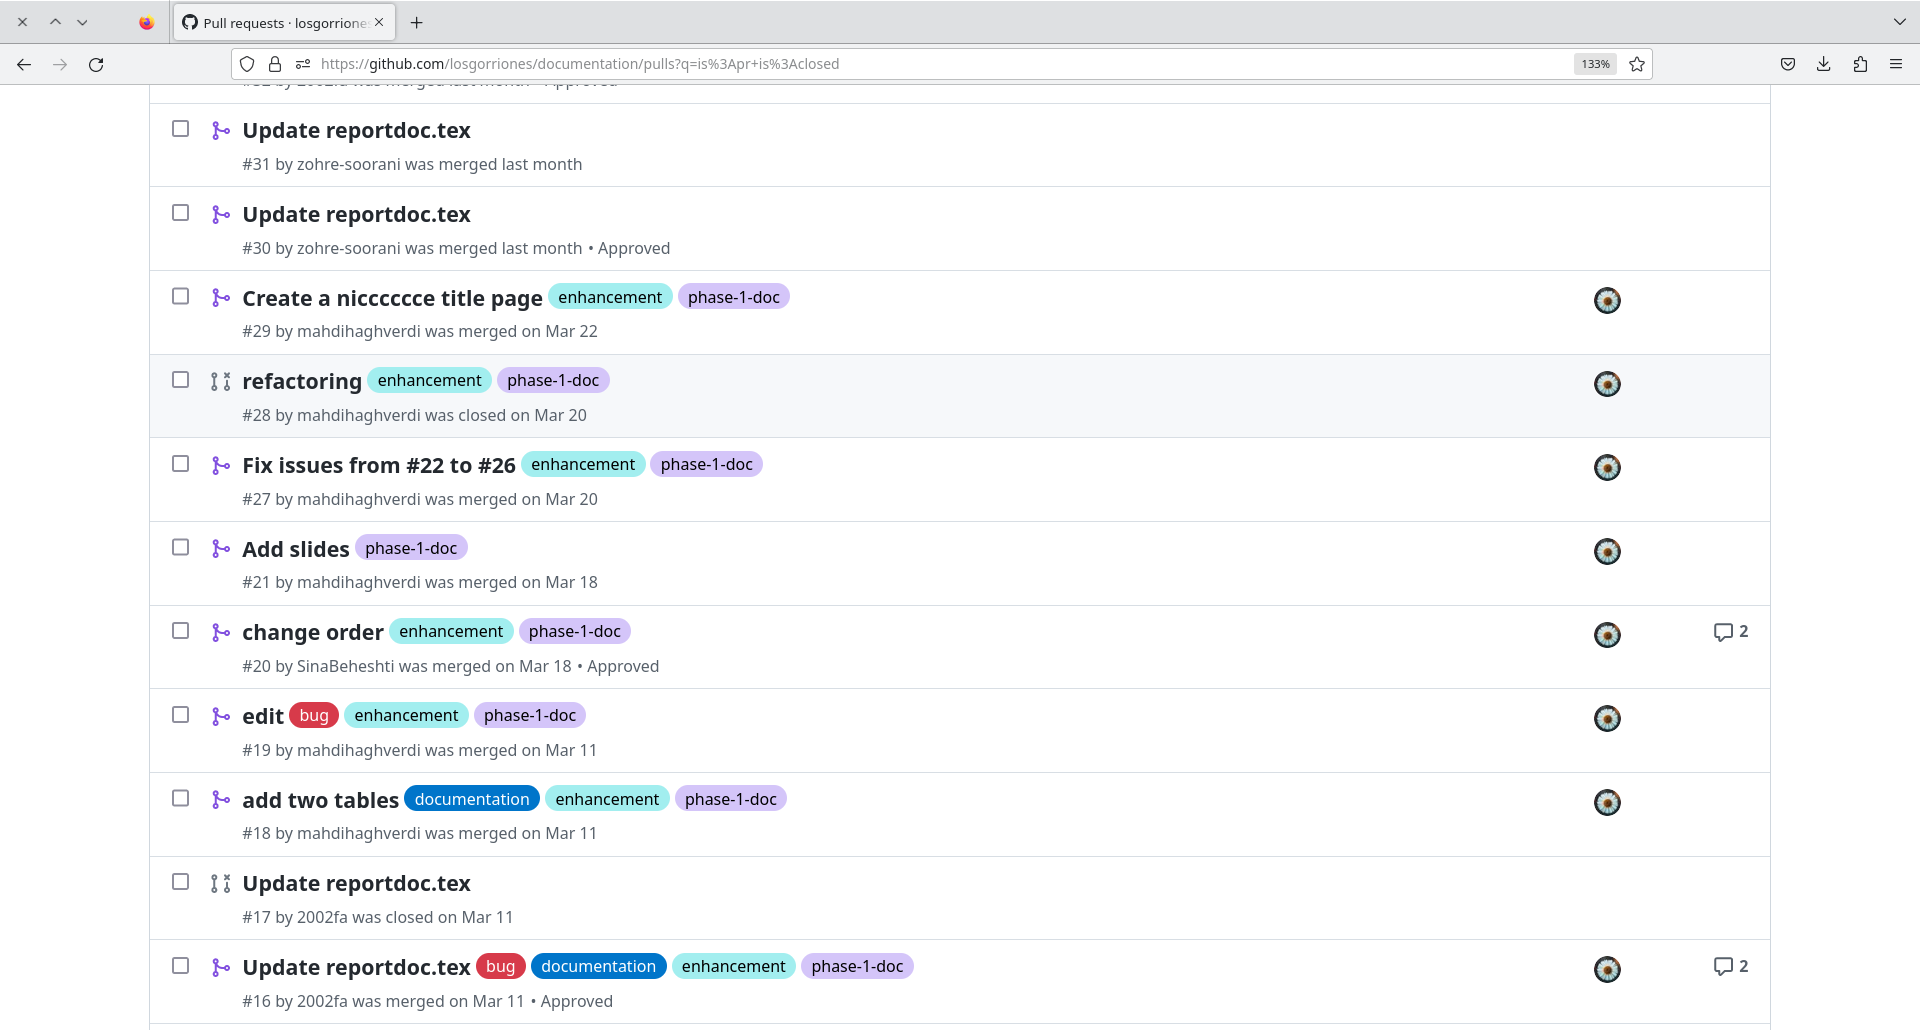
\includegraphics[angle=90, width=\textwidth, height=\textheight]{./images/prs}
\end{center}
\end{figure}

برای گزارش اشکالات در سند هم می‌توان از \lr{Issues} استفاده کرد که امکان تگ‌گذاری و نگهداری همه‌ی آنها در یک مکان را به استفاده کنندگان می‌دهد.
\begin{figure}[H]
	\caption{صفحه‌ی \lr{Issues}}
	\begin{center}
		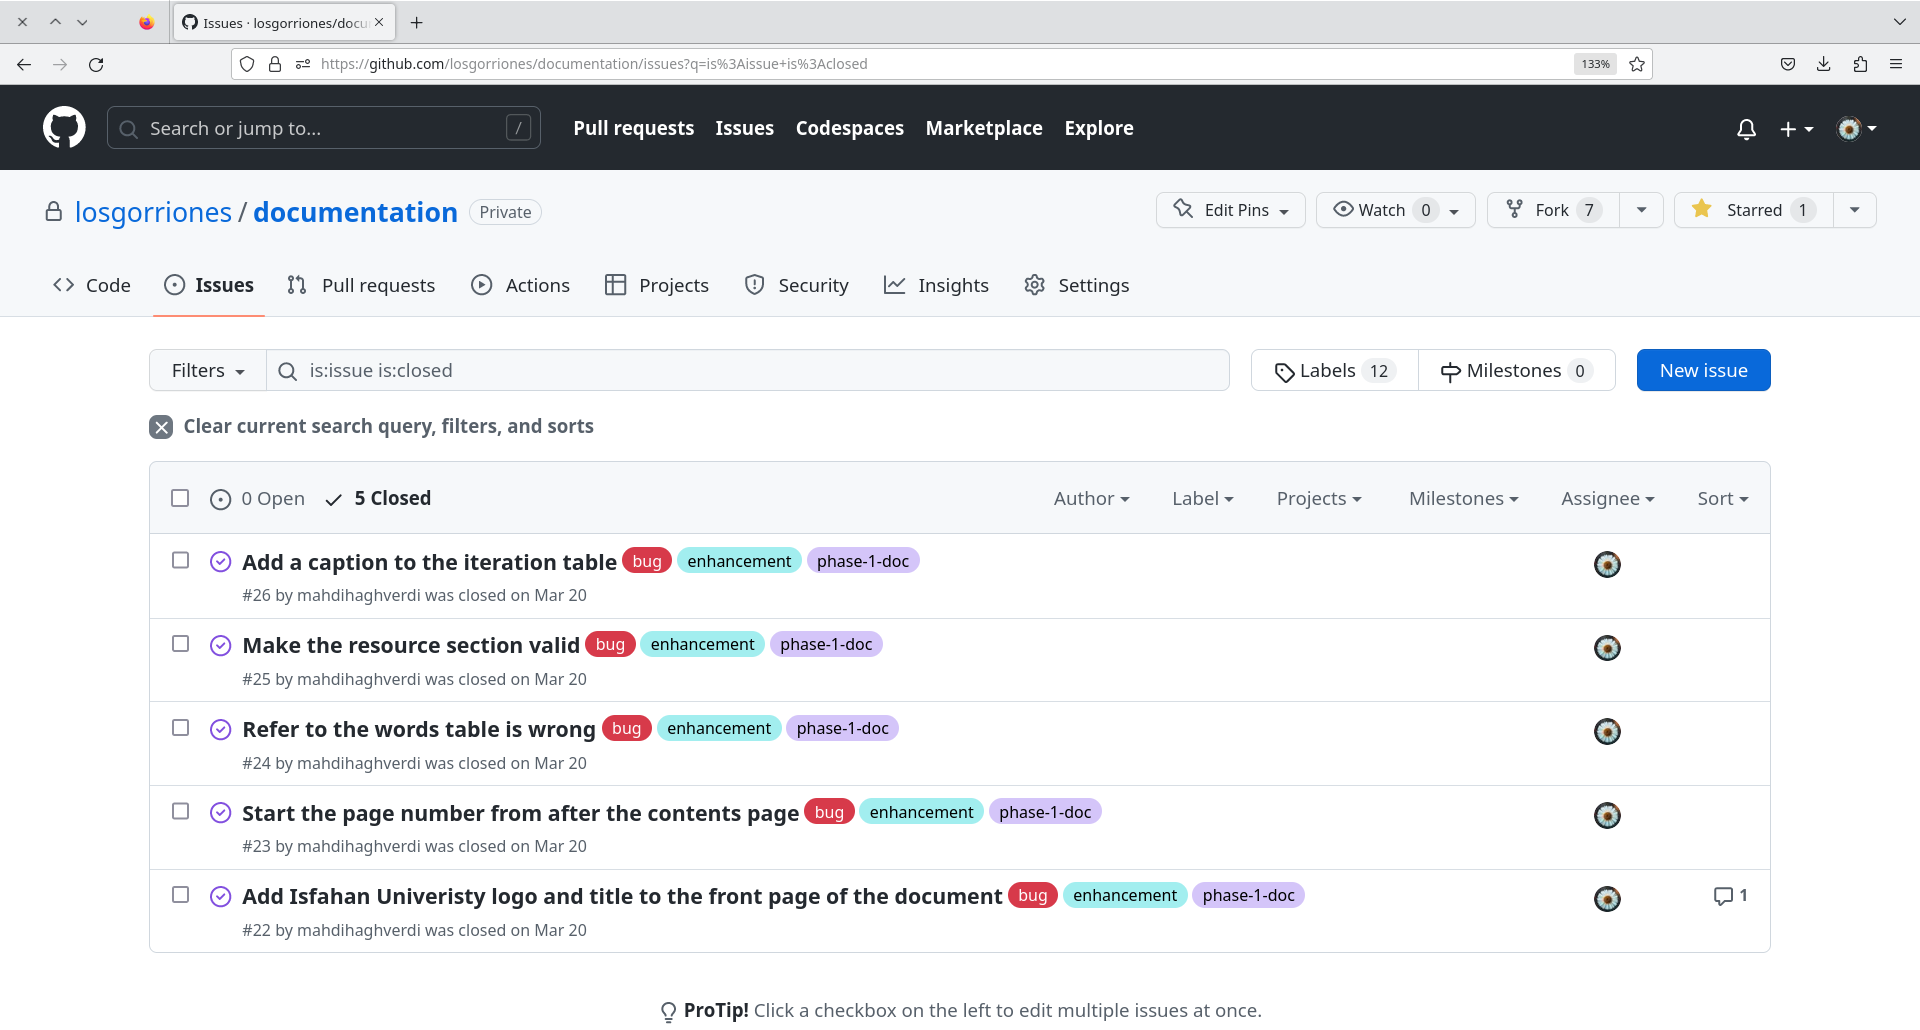
\includegraphics[angle=90, width=0.8\textwidth, height=0.8\textheight]{./images/issues}
	\end{center}
\end{figure}

\subsection{ارائه‌ها}

\begin{latin}
	\begin{center}
		\textit{``People who know what they're talking about, dont't need PowerPoints''} Steve Jobs
	\end{center}
\end{latin}

این درس در سه فاز و هر فاز یک ارائه خلاصه میشه، استاد درس به درس با اسلاید‌هاشون درس میدن، سپس شما شروع به نوشتن سند پروژه‌تون با توجه به مطالب تدریس شده‌ی استاد می‌کنید. چیزی که از همه مهم‌تره کیفیت سند و ارائه‌ی شماست.

ارائه‌ی شما: تمام تلاشی که کردید و تمام نتیجه‌ای که گرفتید رو باید خیلی خلاصه ولی با کلی ذوق، شور و \textbf{کیفیت عالی} به گوش استاد و دیگر همکلاسی‌هاتون برسه.

جمله‌ی استیور جابز رو بخونید، واقعا درسته! داشتن اسلاید‌های خیلی خفن همراه با کلی \lr{Animation} و کلی زرق و برق، هیچ کمکی به ارائه‌تون نمیکنه، بلکه محتوایی که ارائه میدید، ارائه‌تون رو جذاب می‌کنه.

اگه می‌خواید ارائه‌های خیلی خوبی برای زحماتی که کشیدید داشته باشید، به نکات زیر توجه کنید:
\begin{itemize}
	\item 
	{\large سعی کنید بهترین خودتون باشید.}
	
	بله، سعی کنید بهترین خودتون باشید، حتی اگر این فازتون رو اونجوری که می‌خواستید خوب ننوشتید،  اما ارائه‌تون رو عالی تنظیم کنید.
	
	استیو جابز یه حرف دیگه‌ای هم داره که میگه: ارزش هر چیزی به اندازه‌ی معرفی اون چیزه. اگه بتونید یه چیز خوب ارائه کنید (بدونید که هر فاز و هر ارائه نمره‌ی خودشون رو جدا جدا دارن) هم استاد نمره‌ی خوبی بهتون میده و هم بقیه‌ی بچه‌ها تحت تاثیر کار شما قرار میگیرن! در ضمن خودتون هم از کاری که کردید لذت بسیاری خواهید برد و برای ارائه‌ی بعدی یه چیز بهتری ارائه می‌دید.
	
	از تجربه‌ی خودمون براتون بگم: برای فاز اول یکی از اعضای تیم ما اومد اسلاید‌های پروژه رو ساخت و قرار بود که یه روز قبل ارائه ما بخونیمشون رو انتخاب کنیم که چه کسی قراره بره ارائه بده (ارائه‌‌ها معمولا با دو یا سه نفر انجام میشن.) ۳ ساعت قبل ارائه، سینا گفت: بچه‌ها اسلاید‌ها پر!! اسلاید‌ها فقط روی لپ‌تاپش بودن و لپ‌تاپش یه مشکلی براش پیش اومده بود و ما هیچ اسلایدی نداشتیم.\RTLfootnote{پس همیشه یه بک‌اپ از اطلاعاتون داشته باشید}
	توی این اوصاف کاملا وخیم، یک ساعت قبل از ارائه با 
	\lr{Jupyter Notebook}
	یک سری اسلاید خیلی ساده ساختیم.
	قرار شد من و سینا بریم ارائه بدیم. اما ارائه‌ای دادیم که واقعا همه بهمون گفتن چند ساعت تمرین کردید قبلش؟ اسلاید‌هاتون چقدر ساده ولی خوشگل و \textbf{کافی} بودن.
	حتی یه سری از بجه‌ها بهمون گفتن واقعا انگار میخواستید \textit{کارتاپ} رو بنویسید و به یه سازمانی جایی بفروشیدش!
	
	و خب همه‌ی موفقیت این ارائه‌ی خوب خلاصه شد توی این قضیه که \textbf{ما دقیقا می‌دونستیم راجع به چی داریم صحبت می‌کنیم} و \textbf{دقیقا همون رو با اعتماد به نفس} و \textbf{سادگی} به بقیه گفتیم.
	
	\item 
	{\large سعی کنید عمق چیزی که می‌خواهید بگید رو یاد بگیرید}
	
	این واقعا مهمه، استاد هم دقیقا دنبال همینه! می‌خواد بدونه شما اون چیزی که نوشتید و دارید ارائه می‌دید و بلد شدید یا نه. بقیه‌ش دیگه به خلاقیت و مهارت شما برای ارائه دادن و کنترل اون ۱۵ ۲۰ دقیقه‌ای هست که در اختیار دارید.
	
\end{itemize}

\subsection{ارتباط اعضای گروه و برنامه‌ریزی}
اگه بخوایم خیلی ساده بهش نگاه کنیم، گروه شما باید جلسات حضوری زیادی داشته باشه. ارتباط رودرو و کار گروهی کنار هم خیلی \lr{effective}‌تر از کار مجازی‌ هست.

اما خب بالاخره ارتباط مجازی هم نیازه. فعالیت اصلی تیم‌مون توی تلگرام و گروه‌مون بود و کار‌های برنامه‌ریزی و تعریف کارها توی ترلو بود.

این هم عکسی از ترلوي فاز اول پروژه‌ی ما بود (تصویر \ref{trello})
\begin{figure}[H]
	\begin{center}
		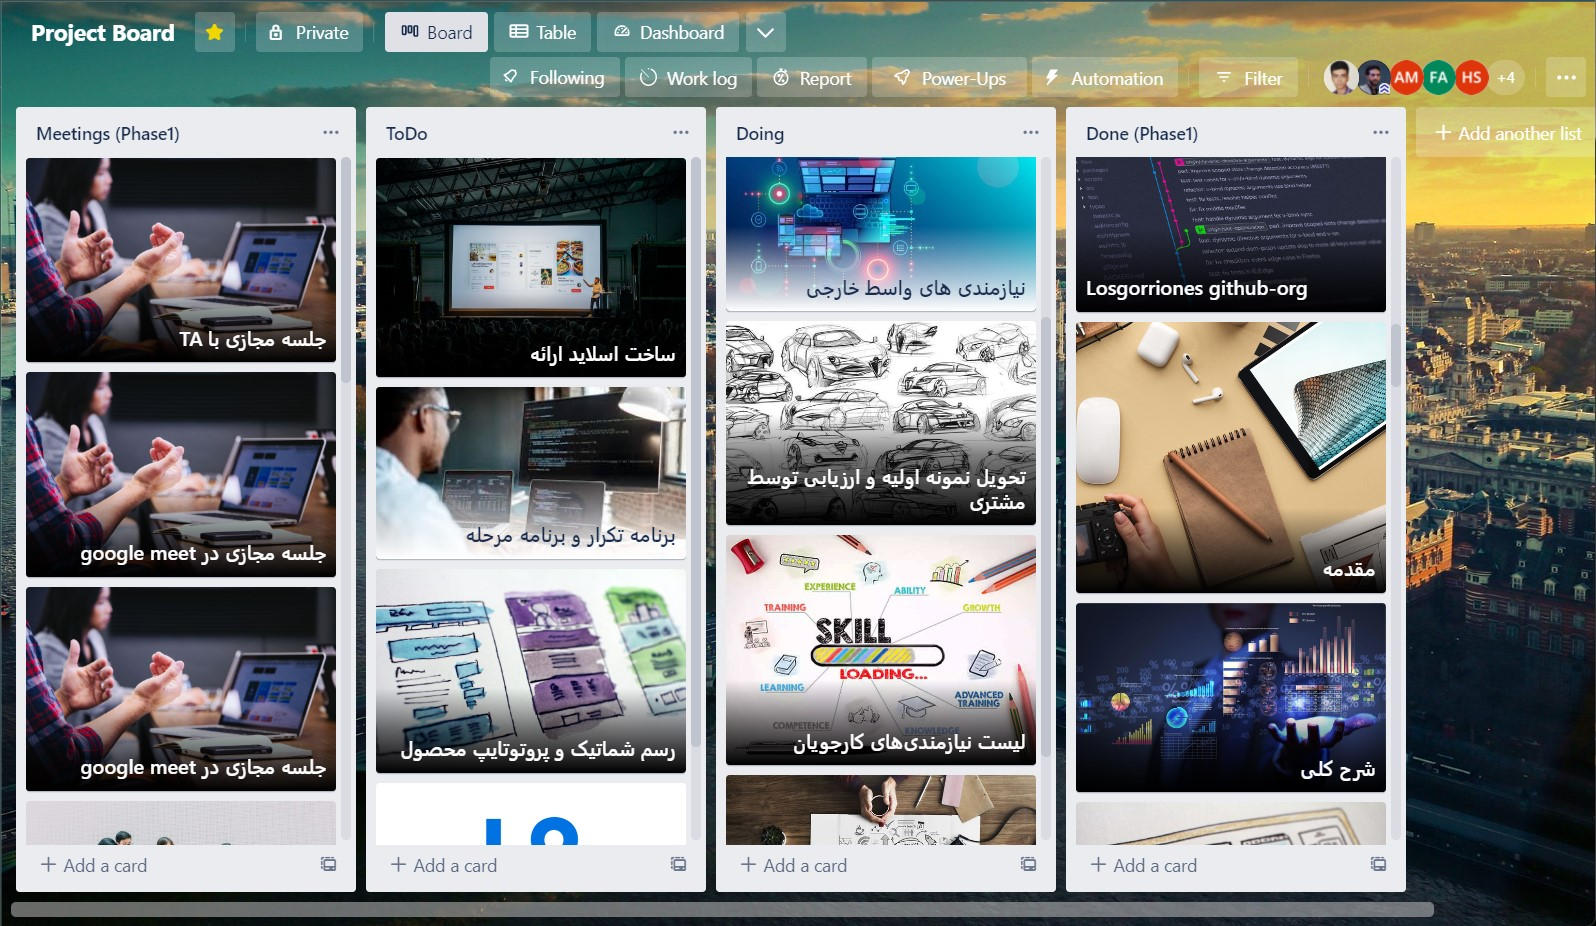
\includegraphics[width=\textwidth, angle=90, height=\textheight]{./images/trello}
	\end{center}
\caption{تصویر ترلو فاز یک}
\label{trello}
\end{figure}

\begin{flushleft}
	موفق باشید.
\end{flushleft}